\documentclass[12pt,a4paper]{jsarticle}
\setlength{\topmargin}{-15mm}
\setlength{\oddsidemargin}{-15mm}
\setlength{\evensidemargin}{-10mm}
\setlength{\textwidth}{180mm}
\setlength{\textheight}{260mm}

\usepackage[top=15truemm,bottom=25truemm,left=20truemm,right=20truemm]{geometry}
\usepackage[latin1]{inputenc}
\usepackage{amsmath}
\usepackage{amsfonts}
\usepackage{amssymb}
\usepackage[dvipdfmx]{graphicx}
\usepackage{listings}
\usepackage{listings,jvlisting}
\usepackage{geometry}
\usepackage[dvipdfmx]{hyperref}
\usepackage{pxjahyper}
\hypersetup
{setpagesize=false,
 bookmarksnumbered=true,
 bookmarksopen=true,
 colorlinks=true,
 linkcolor=blue,
 citecolor=blue,
}

\lstset{
basicstyle={\ttfamily},
identifierstyle={\small},
commentstyle={\smallitshape},
keywordstyle={\small\bfseries},
ndkeywordstyle={\small},
stringstyle={\small\ttfamily},
frame={tb},
breaklines=true,
columns=[l]{fullflexible},
xrightmargin=0zw,
xleftmargin=3zw,
numberstyle={\scriptsize},
stepnumber=1,
numbersep=1zw,
lineskip=-0.5ex
}

\title{Airfoil Adjuster の使い方}
\author{}
\date{}

\begin{document}
\maketitle
\section*{【座標データの作成】}
\begin{enumerate}
    \item "airfoil\_ajuster.exe"のあるフォルダ内に"original"と"result"の2つのフォルダを作成してください。
          \begin{figure}[htbp]
              \begin{center}
                  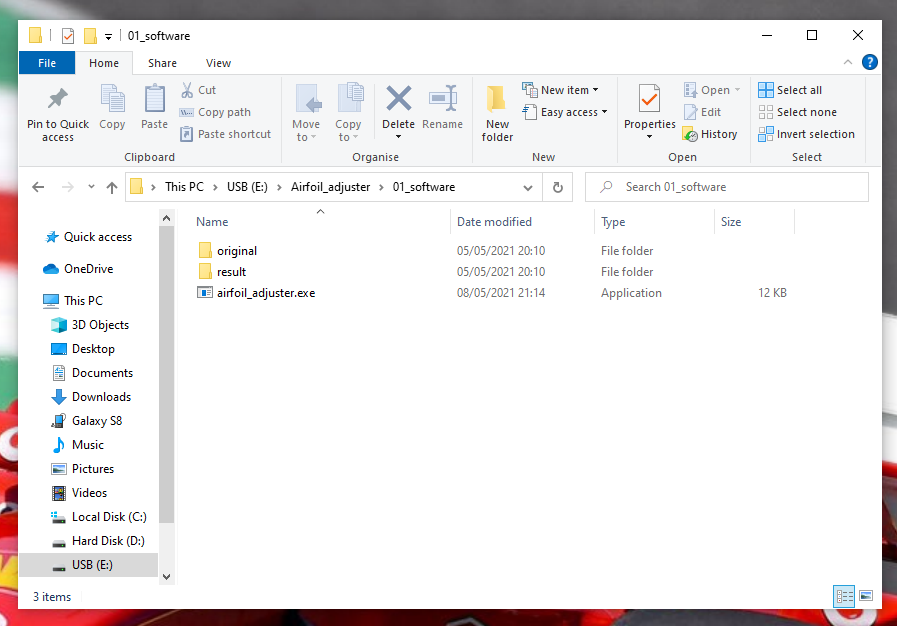
\includegraphics[width=110mm]{images/image_1.png}
              \end{center}
          \end{figure}
    \item "original"のフォルダ内に使用したい翼型の座標を".txt"ファイル形式で保存します。\\
          ● 使用する .txt ファイルの1行目は読み飛ばされるようにしているので,翼型名を書いておくと良いです.\\
          ● 下図のように,1行目に”翼型名”,2行目以降にx,y座標が表示されている形式で保存してください.
          \begin{figure}[htbp]
              \begin{center}
                  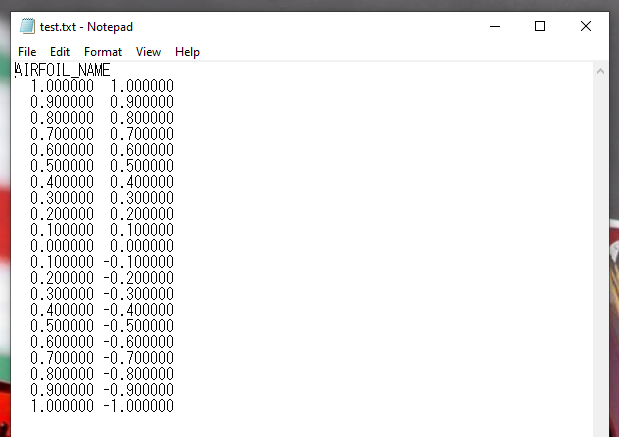
\includegraphics[width=110mm]{images/image_3.png}
              \end{center}
          \end{figure} \\
          \newpage
    \item "airfoil\_ajuster.exe"をダブルクリックして起動し、指示に従って翼型のファイル名と任意の翼弦長を入力します.\\
          ● このとき、".txt"は入力しなくて大丈夫です. 例)"20-32c.txt" を使用する → "20-32c" のみ入力\\
          ● 翼弦長は半角で単位は"mm"で入力してください。\\
          ● ファイルの読み込みに失敗した場合は、指示にしたがってプログラムを終了し最初からやり直してください。\\
    \item プログラムが正常に動作している場合は、以下の画像のように結果が表示されます。
          \\確認後、指示にしたがって終了してください。\\
          \begin{figure}[htbp]
              \begin{center}
                  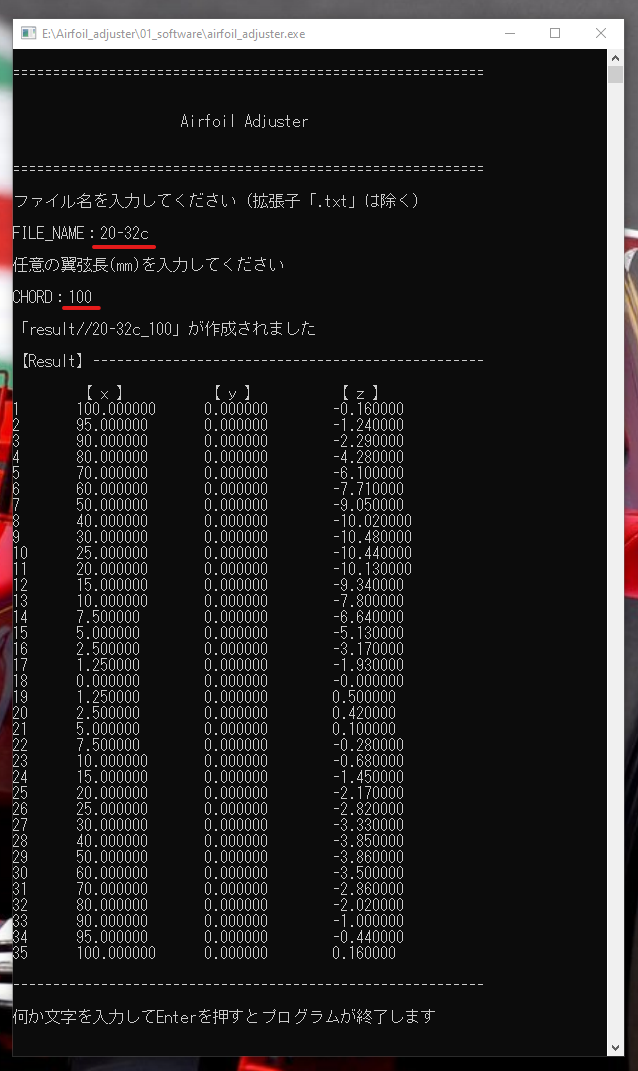
\includegraphics[width=125mm]{images/image_8.png}
              \end{center}
          \end{figure} \\
    \item "result"のフォルダに "ファイル名"\_"翼弦長" のフォルダが作成され,\\
          その中に"asc","txt","csv"形式で翼型の座標が保存されます。\\
          \begin{figure}[htbp]
              \begin{center}
                  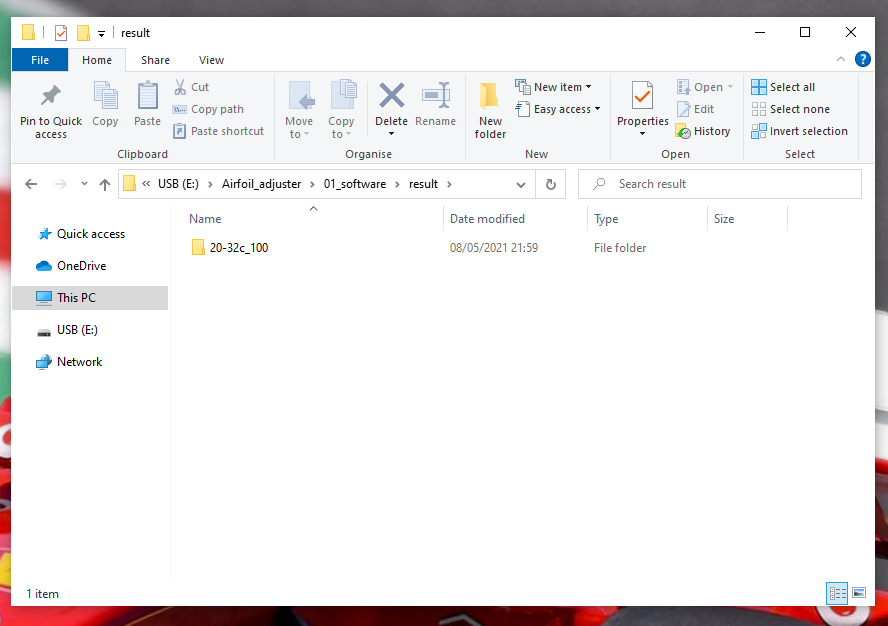
\includegraphics[width=120mm]{images/image_9.png}
              \end{center}
          \end{figure} \\
          \begin{figure}[htbp]
              \begin{center}
                  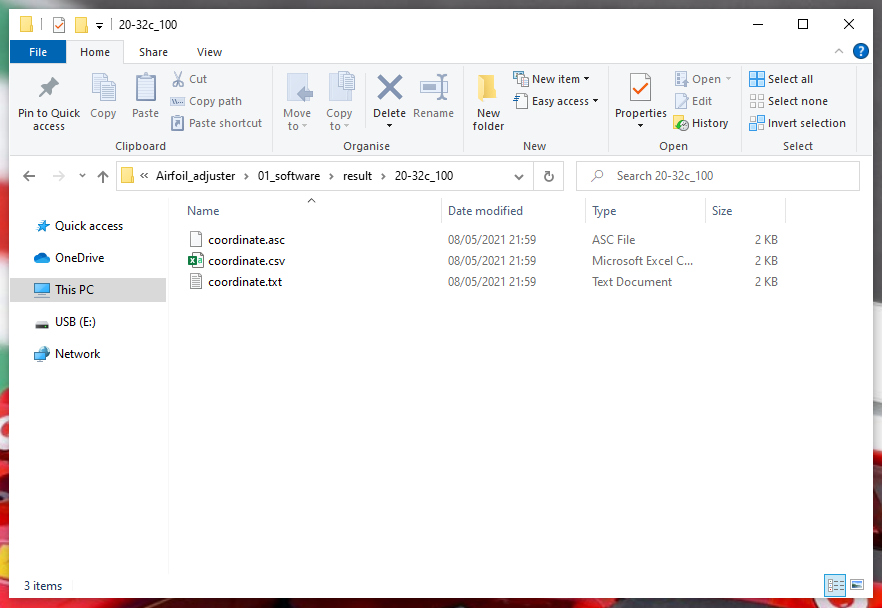
\includegraphics[width=120mm]{images/image_10.png}
              \end{center}
          \end{figure} \\
\end{enumerate}
\newpage
\section*{【翼型に使用する.txt データついて】}
おなじみの"\href{{http://airfoiltools.com}}{Airfoil Tools}"を使用します.\\
"Airfoil search"を使用して好きな翼型を選んでください.
\begin{figure}[htbp]
    \begin{center}
        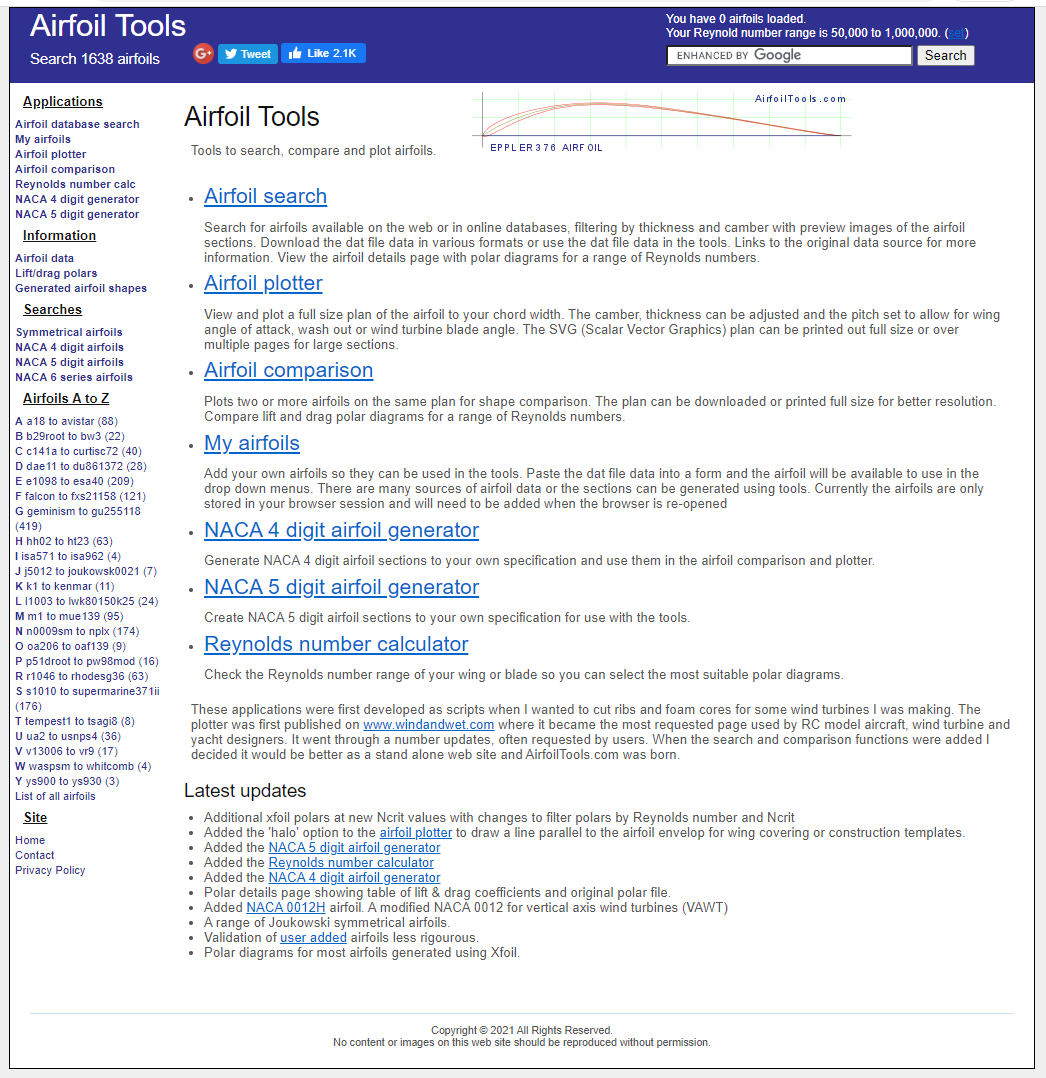
\includegraphics[width=120mm]{images/image_4.png}
    \end{center}
\end{figure} \\
その後,下図のように希望の翼型の"Airfoil details"に進んでください.
\begin{figure}[htbp]
    \begin{center}
        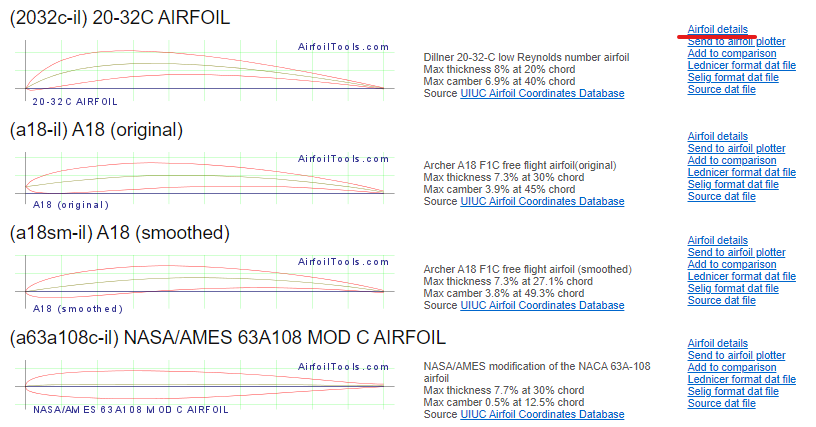
\includegraphics[width=120mm]{images/image_5.png}
    \end{center}
\end{figure} \\
\newpage
次に,"Seling format dat file"に進みます.
\begin{figure}[htbp]
    \begin{center}
        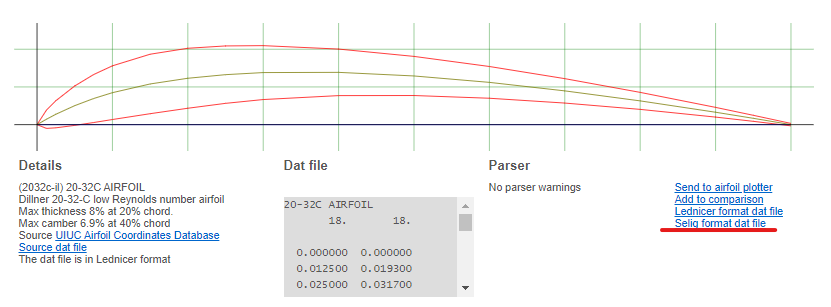
\includegraphics[width=120mm]{images/image_6.png}
    \end{center}
\end{figure} \\
ブラウザ上で1行目に翼形名,2行目以降に単位長さで示された座標データ(0から1まで)が表示されます.
この画面上で"ctrl + s"を押すと,".txt"ファイル形式で保存ができるので"original"のフォルダに保存してください.\\
※ .datファイル形式で保存される場合は,拡張子を".dat" から”.txt”に変更してもらえれば大丈夫だと思います.
\begin{figure}[htbp]
    \begin{center}
        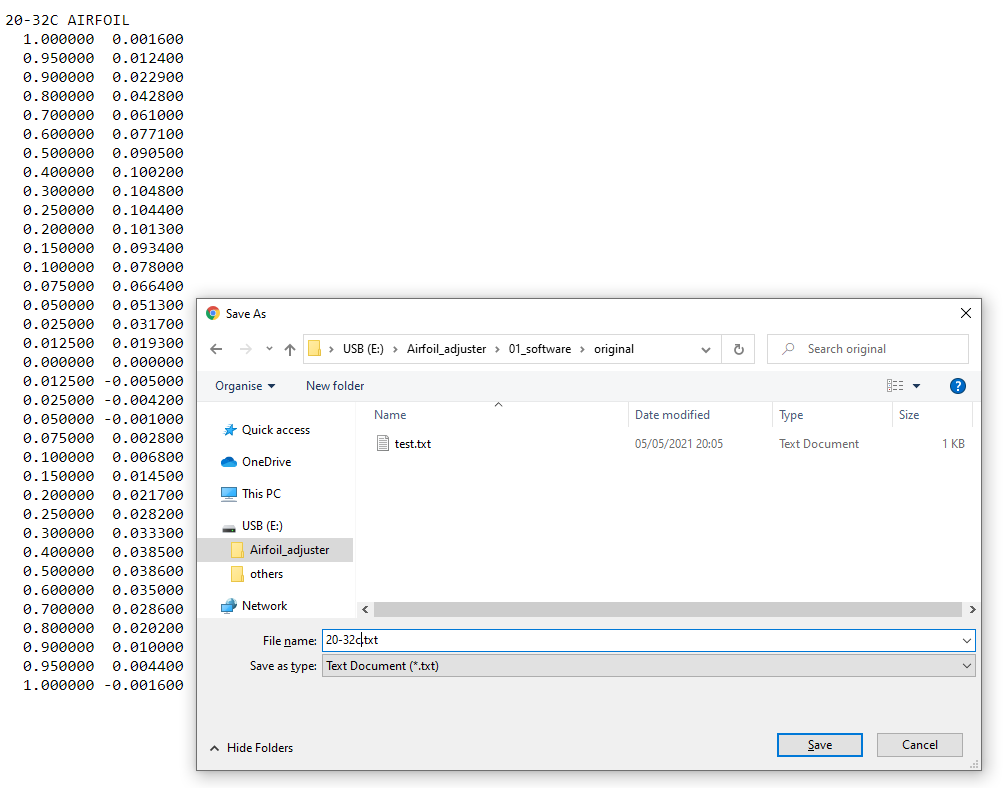
\includegraphics[width=120mm]{images/image_7.png}
    \end{center}
\end{figure} \\
\newpage
\section*{【ソースコード】}
\small
\begin{lstlisting}
/******************************************************************************
PROGRAM NAME : airfoil_adjuster.cpp
AUTHER : Masatsugu Kitadai
DATE : 5/5/2021
******************************************************************************/
#include <stdio.h>
#include <stdlib.h>
#include <string.h>
#include <sys/stat.h>
#include <math.h>
#include <direct.h>
#define num 1000

double coordinate[num][3];
char airfoil_name[100];
char buf[128];
char read_file[100];
char output_file_csv[100];
char output_file_xlsx[100];
char output_file_txt[100];
char output_file_asc[100];
char folder_name[100];
char space[1000];

FILE* read;
FILE* output;
/*********************************   MAIN   *********************************/
int main()
{
   // デザイン
    printf("\n===========================================================\n\n");
    printf("\n                     Airfoil Adjuster                      \n\n");
    printf("\n===========================================================\n\n");

    int i, chord;
    double x, y;

    i = 0;

    // 読み込むファイルを指定する
    printf("ファイル名を入力してください(拡張子「.txt」は除く)\n\n");
    printf("FILE_NAME:");
    scanf("%s", airfoil_name);

    // 入力・出力ファイル名の指定

    sprintf(read_file, "original//%s.txt", airfoil_name);

    // 読み込むファイルを開く

    read = fopen(read_file, "r");
    if (read == NULL)
    {
        printf("\nファイルが開けません\n");
        printf("最初からやり直してください\n\n");
        printf("何か文字を入力してEnterを押すとプログラムが終了します\n");
        scanf("%s", space);
        exit(0);
    }

    // 最初の1行を読み飛ばす

    fgets(buf, sizeof(buf), read);

    // 最後の行以外を読み込み,配列に格納する

    while (fscanf(read, "%lf %lf", &x, &y) != EOF)
    {
        i = i + 1;
        coordinate[i][1] = x;
        coordinate[i][2] = 0;
        coordinate[i][3] = y;
    }

    // "EOF"で判別できない最後の行を読み込む

    fscanf(read, "%lf %lf", &x, &y);
    i = i + 1;
    coordinate[i][1] = x;
    coordinate[i][2] = 0;
    coordinate[i][3] = y;

    fclose(read);

    // 配列の大きさを決定

    int data_long;
    data_long = i;

    // 翼弦長を指定する
    printf("\n任意の翼弦長(mm)を入力してください\n\n");
    printf("CHORD:");
    scanf("%d", &chord);

    // "z"座標の上下を反転させる

    for (i = 0; i < data_long; i++)
    {
        coordinate[i][3] = (-1.0) * coordinate[i][3];
    }

    // 指定された翼弦長に修正する

    for (i = 1; i < data_long; i++)
    {
        coordinate[i][1] = chord * coordinate[i][1];
        coordinate[i][3] = chord * coordinate[i][3];
    }

    // 保存するディレクトリを作成

    sprintf(folder_name, "result//%s_%d", airfoil_name, chord);

   if (_mkdir(folder_name) == 0)
   {
       printf("\n「%s」が作成されました\n", folder_name);
   }
   else 
   {
       printf("\n「%s」はすでに作成されています\n", folder_name);
   }

    // 書き込むファイルの名前を指定する

    sprintf(output_file_csv, "result//%s_%d//coordinate.csv", airfoil_name, chord);
// sprintf(output_file_xlsx, "result//%s_%d//coordinate.xlsx", airfoil_name, chord);
    sprintf(output_file_txt, "result//%s_%d//coordinate.txt", airfoil_name, chord);
    sprintf(output_file_asc, "result//%s_%d//coordinate.asc", airfoil_name, chord);

    // それぞれのファイルに書き込む

    //csv ファイル

    output = fopen(output_file_csv, "w");

    for (i = 1; i < data_long; i++)
    {
        fprintf(output, "X,%lf,Y,%lf,Z,%lf\n", coordinate[i][1], coordinate[i][2], coordinate[i][3]);
    }

    fclose(output);

    //xlsx ファイル
/*
    output = fopen(output_file_xlsx, "w");

    for (i = 1; i < data_long; i++)
    {
        fprintf(output, "X,%lf,Y,%lf,Z,%lf\n", coordinate[i][1], coordinate[i][2], coordinate[i][3]);
    }

    fclose(output);
 */

    //txt ファイル

    output = fopen(output_file_txt, "w");

    for (i = 1; i < data_long; i++)
    {
        fprintf(output, "X\t%lf\tY\t%lf\tZ\t%lf\n", coordinate[i][1], coordinate[i][2], coordinate[i][3]);
    }

    fclose(output);

    //asc ファイル

    output = fopen(output_file_asc, "w");

    for (i = 1; i < data_long; i++)
    {
        fprintf(output, "X\t%lf\tY\t%lf\tZ\t%lf\n", coordinate[i][1], coordinate[i][2], coordinate[i][3]);
    }

    fclose(output);

    // アプリケーションに出力

    printf("\n【Result】-------------------------------------------------\n\n");

    printf("\t【 x 】\t\t【 y 】\t\t【 z 】\n");

    for (i = 1; i < data_long; i++)
    {
        printf("%d\t%lf\t%lf\t%lf\n", i, coordinate[i][1], coordinate[i][2], coordinate[i][3]);
    }

    printf("\n-----------------------------------------------------------\n\n");

    printf("何か文字を入力してEnterを押すとプログラムが終了します\n");
    scanf("%s", space);

    return (0);
}
\end{lstlisting}
\end{document}